\documentclass[11pt,a4paper]{article}
\usepackage[margin=2.4cm]{geometry}
\usepackage{amsmath,amssymb,booktabs,hyperref,graphicx}
\newcommand{\dt}{\Delta t}
\makeatletter\newcommand{\tabinput}[1]{\@@input #1 }\makeatother
\newcommand{\code}[1]{\texttt{\small #1}}
\title{Split-explicit time integration for a mountain wave:\\
MIS, RK3, exponential and Lawson methods\\ with frozen and linearized fast parts}
\author{MultiRate.jl}
\date{\today}
\begin{document}
\maketitle

\begin{abstract}
We compare split-explicit time integrators for the compressible Euler equations on a
terrain-following finite-volume grid, using the hydrostatic mountain wave over the Agnesi hill
($a=10$\,km) as test case. The fast part is integrated by a HEVI loop that couples horizontal
St\"ormer--Verlet half steps with a vertically implicit Crank--Nicolson step. Four published MIS
methods are compared with the Wicker--Skamarock RK3, two exponential (ETD) methods and a Lawson
method, each for four ways of splitting the right-hand side: three \emph{frozen} splittings (full
pressure, frozen product form, extended system with the Exner pressure as an additional prognostic
variable) and the classical \emph{linearized} splitting $N=L_n+(N-L_n)$. Accuracy is measured
against RK4 of the same semi-discrete operator, together with the largest stable time step and the
dependence on the number of small steps.
\end{abstract}

\tableofcontents

%======================================================================
\section{Introduction}
In the compressible equations of atmospheric dynamics the fastest waves, sound waves with
$c\approx350$\,m/s, carry almost no meteorologically relevant energy, while the flow of interest
moves with $10$--$50$\,m/s. An explicit method for the whole system is limited by the acoustic
Courant number and wastes most of its work on the acoustic modes. \emph{Split-explicit} methods
integrate the terms responsible for the sound waves with small time steps $\Delta\tau$ and the
remaining (``slow'') terms --- advection, in our case also all nonlinear transport --- with a large
step $\dt$. The idea goes back to Klemp and Wilhelmson (1978); the Runge--Kutta form of Wicker and
Skamarock (2002), RK3 with forward--backward small steps, is the time integrator of WRF and many other
models (Skamarock and Klemp 1992, 1994; Klemp, Skamarock and Dudhia 2007).

Multirate infinitesimal step (MIS) methods (Wensch, Knoth and Galant 2009; Knoth and Wensch 2014)
generalize this construction. Each stage solves an ordinary differential equation for the fast part,
whose initial value and forcing are linear combinations of the previous stages; the coefficients
$(\alpha,\beta,\gamma)$ are free parameters that can be chosen for order and stability. RK3 is the MIS
method with $\alpha=\gamma=0$. Order conditions are derived assuming that the fast stages are solved
exactly (``infinitesimal step''); in practice they are integrated with a few small steps. Four-stage
MIS methods of order 3 (MIS4a) and five-stage methods with large stability regions (MIS54, Bauer and
Knoth 2021) are available.

Exponential integrators (Hochbruck and Ostermann 2010) follow a related idea: the fast part $L$ is
integrated exactly, through the matrix functions $e^{\tau L}$ and $\varphi_k(\tau L)$, and the slow
part enters as a polynomial forcing. In stage form (``exponential time differencing'', ETD; Cox and
Matthews 2002, Krogstad 2005) each stage is again a fast ODE with a forcing that is polynomial in
time, and the $\varphi$-functions are replaced by a fast integrator; this makes ETD methods
split-explicit methods of their own kind. Lawson methods (Lawson 1967) integrate in the frame of the
fast flow (integrating factor). With exact fast stages and commuting fast and slow operators both
reproduce the slow Runge--Kutta method on the slow part; in general they do not.

The splitting itself is a design decision. The classical approach linearizes the fast part about the
state at the beginning of the large step, $N(q)=L_nq+(N(q)-L_nq)$, with a constant matrix $L_n$
(\emph{linearized} splitting). Alternatively the right-hand side can be written as
$N(q)=F(q,q)$ with a first argument \emph{frozen} at the stage values and a second one evolving in the
fast integration (Knoth and Wensch, B-series and split-explicit methods); the fast part may then be
nonlinear and its coefficients come from the stages, not from $q^n$. We compare three frozen forms:
the full pressure $p(\Theta)$ in the fast part, the frozen product form $(\partial p/\partial\Theta)_f
\,\delta\Theta$, and an \emph{extended system} in which the Exner pressure $\pi$ is an additional
prognostic variable with its own (consistent) evolution equation, so that the pressure gradient is
the product $c_p\Theta\nabla\pi$ with frozen $\Theta$ and the fast part is linear in the evolving
variables.

The test case is the hydrostatic mountain wave of Gallus and Klemp (2000) on a terrain-following
(Gal-Chen and Somerville 1975) grid. It contains the two features that make split-explicit
integration delicate: vertically propagating gravity waves forced by the orography (slow, but with
vertical structure on the grid scale) and the acoustic transients excited by the impulsive start and
by the metric terms of the coordinate transformation.

%======================================================================
\section{Spatial discretization}
\paragraph{Grid.} Periodic channel $[0,L_x]$, model top $H$; Gal-Chen coordinate
$z=z_s(x)+\eta J(x)$, $J=1-z_s/H$, cells uniform in $(x,\eta)$; Arakawa C-grid: $\rho$, $\Theta=\rho\theta$
(and $\pi$) at the cell centres, $U=\rho u$ at the x-faces, $W=\rho w$ at the interior $\eta$-faces
($W=0$ at the ground and the top is replaced by the kinematic condition through the contravariant
flux).
\paragraph{Conservation laws.} Mass and $\Theta$ in flux form,
\[
\partial_t\rho=-\frac1J\Big[\delta_x(J_xU)+\delta_\eta\Omega\Big],\qquad
\partial_t\Theta=-\frac1J\Big[\delta_x(\theta_xJ_xU)+\delta_\eta(\theta_\eta\Omega)\Big],\qquad
\Omega=W-z_x\bar U,
\]
$\bar U$ the four-point mean, $\Omega=0$ at the ground and the top. The face values $\theta_x$,
$\theta_\eta$ are pseudo third-order upwind values (Jähn et al.\ 2015), the momentum advection uses the
shift technique (Hicken et al.\ 2005; Jähn et al.\ 2015).
\paragraph{Pressure gradient} in the metric form
\[
-\partial_xp|_z=-\frac1{J_x}\Big[\delta_x(Jp)-\delta_\eta(z_xp_\sigma)\Big],\qquad
-\partial_zp=-\frac{\delta_\eta p}{J\Delta\eta},
\]
$p_\sigma$ the mean at the $\eta$-faces, quadratically extrapolated at the ground and the top (so that
the hydrostatic part has interior truncation error); gravity $-g\bar\rho$ at the $W$ faces. No
reference state is subtracted. A Rayleigh layer damps $W$ above $z_D$.
\paragraph{Discrete balance.} Each column is initialized in discrete hydrostatic balance of the $W$
row of the respective form (rest-state residual $|N_W|\le6\cdot10^{-13}$); the remaining
$|N_U|\approx2$--$4\cdot10^{-5}$ is the truncation error of the horizontal pressure gradient on the
sloping coordinate surfaces.

%======================================================================
\section{Splittings and extended systems}
The semi-discrete system is $q'=N(q)$, $q=(\rho,U,W,\Theta)$. All split-explicit methods need a fast
part. We write $N(q)=F(q,q)$ with
\[
F(y,z)=F_f(C(y),z)+S(y),
\]
$S$ the slow part (momentum advection, $y$ only) and $F_f$ the fast part, which depends on the
evolving $z$ and on coefficients $C(y)$ frozen from $y$, linearly in $C$ (so that the MIS combination
of stages is a combination of the $C$).
\begin{itemize}
\item \textbf{Frozen, full pressure} (\code{gradp}): $C=(\theta_x,\theta_\eta)$, the face values of
$\theta$; $F_f$ contains the mass and $\Theta$ fluxes of $z$ with frozen $\theta_f$, the full
pressure $p(\Theta_z)$ and gravity. Nonlinear in $z$ through $p(\Theta)$; the vertical implicit step
uses an approximate Jacobian.
\item \textbf{Frozen product form} (\code{product}): additionally the face derivative
$P_f=(\gamma p/\Theta)_f(y)$ is frozen, $-\partial_xp\approx-P_f\,\partial_x\Theta|_z$; $F_f$ is linear in
$z$, the vertical step is exactly Crank--Nicolson. On the terrain grid $N(q)=F(q,q)$ defines the
operator (it differs from the full-pressure one by the product rule).
\item \textbf{Extended system} (\code{exner}): the Exner pressure $\pi=(p/p_0)^{R/c_p}$ is an additional
prognostic variable with
\[
\partial_t\pi=\frac{\partial\pi}{\partial\Theta}\partial_t\Theta,\qquad
\nabla p=c_p\Theta\nabla\pi\quad\text{(exact)},
\]
frozen coefficients $\kappa_f=(\partial\pi/\partial\Theta)\theta_f$ per face and neighbour and the face
mean $c_p\bar\Theta_f$ in the momentum rows. $F_f$ is linear in $z=(\rho,U,W,\Theta,\pi)$. The system
keeps $\pi=\pi(\Theta)$ in continuous time; after every large step $\pi$ is reset from $\Theta$.
\item \textbf{Linearized} (\code{linear}): $N(q)=L_nq+(N(q)-L_nq)$, $L_n$ the Jacobian-like fast
operator frozen at $q^n$ and refrozen every large step; the slow part is $N-L_n$ evaluated at the
stages; $N$ is the full-pressure operator.
\end{itemize}

%======================================================================
\section{Time integration schemes}
\paragraph{MIS.} With $Y_1=q^n$, stage $i=2,\dots,s+1$ solves over $\tau\in[0,d_i\dt]$, $d_i=\sum_j\beta_{ij}$,
\[
Z'=F_f\Big(\sum_j w_{ij}C(Y_j),Z\Big)+\sum_jw_{ij}S(Y_j)+\sum_j\frac{\gamma_{ij}}{d_i\dt}(Y_j-q^n),\qquad
Z(0)=q^n+\sum_j\alpha_{ij}(Y_j-q^n),
\]
$w_{ij}=\beta_{ij}/d_i$, $Y_i=Z(d_i\dt)$, with $\lceil d_in_{\rm sub}\rceil$ small steps. Published methods
used here: MIS2 (2nd order), MIS3C, MIS4a (Knoth and Wensch 2014) and MIS54 (Bauer and Knoth 2021).
With a frozen coefficient the order of MIS54 and MIS4a drops to 2 (order conditions of the bicoloured
B-series); MISF53 and the application-specific MIS\_FV53 restore order 3.
\paragraph{RK3 (Wicker--Skamarock).} MIS with $\alpha=\gamma=0$, $\beta=\mathrm{diag}(1/3,1/2,1)$: every
stage restarts from $q^n$; order 2 for nonlinear fast parts.
\paragraph{ETD3, ETD4.} Stage form of exponential RK methods: stage $i$ integrates from $q^n$ over
$c_i\dt$
\[
Z'=F_f(C(q^n),Z)+\sum_{j\le i}\sum_kP_{ijk}\,(\tau/c_i\dt)^{k-1}\,\tilde S(Y_j),\qquad
\tilde S(Y)=N(Y)-F_f(C(q^n),Y),
\]
with the polynomial coefficients $P$ of the $\varphi$-function representation: ETD3 is the
Cox--Matthews ETDRK3 ($c=\tfrac12,1,1$), ETD4 Krogstad's ETDRK4 ($c=\tfrac12,\tfrac12,1,1$). The fast
part is frozen at $q^n$ (frozen forms) or is $L_n$ (linearized).
\paragraph{Lawson4.} Integrating-factor form of classical RK4: the increments $\dt\,a_{ij}\tilde S(Y_j)$ are
propagated by the fast flow between the nodes $c_j\to c_i$; with a nonlinear fast flow the order drops
to 2.
\paragraph{Number of small steps.} For a stage of length $c\,\dt$, $\lceil c\,n_{\rm sub}\rceil$ small
steps, $n_{\rm sub}=\lceil\dt/\Delta\tau_{\rm ac}\rceil$ (times a factor in Section~\ref{sec:nsub}),
$\Delta\tau_{\rm ac}=0.85\cdot0.92\,\Delta x/c$ (4.3\,s here). Fast work per large step: $\sum_id_i$
(MIS), $\sum_ic_i$ (ETD), the node propagations (Lawson).

%======================================================================
\section{The fast integrator: St\"ormer--Verlet coupled with HEVI}
The fast part is split into a horizontal part $F_h$ (horizontal fluxes, the horizontal part
$-z_x\bar U$ of $\Omega$, the horizontal pressure gradient with its metric term, and all constant
forcings) and a vertical part $F_v$ (the $W$ part of the $\eta$-flux, the vertical pressure gradient
and gravity). One small step $\Delta\tau$ is the symmetric composition
\[
\Phi_{\Delta\tau}=H_{\Delta\tau/2}\circ V_{\Delta\tau}\circ H_{\Delta\tau/2},
\]
where $H$ is a St\"ormer--Verlet step of the horizontal part (thermodynamic rows a quarter step,
momentum a half step, thermodynamic rows a quarter step: position Verlet; Hairer, Lubich and Wanner
2006) and $V$ the linearly implicit Crank--Nicolson step
\[
z\leftarrow z+\Big(I-\tfrac{\Delta\tau}2J_v\Big)^{-1}\Delta\tau\,F_v(z)
\]
of the vertical part, solved column by column: $\rho$, $\Theta$ (and $\pi$) are eliminated, leaving a
tridiagonal system for $W$ (as in WRF). For the linear fast parts (product form, extended system) $V$
is exactly Crank--Nicolson. The composition is symmetric and of second order; the horizontal part
is limited by the horizontal acoustic Courant number, the vertical one is unconditionally stable,
which removes the restriction $\Delta\tau<\Delta z/c$ ($\Delta z/c\approx0.6$\,s here, against
$\Delta\tau_{\rm ac}=4.3$\,s). No divergence damping (extrapolation) is used in this study.

%======================================================================
\section{Test case}
Agnesi hill $h(x)=h_0/(1+(x-x_m)^2/a^2)$, $h_0=400$\,m, $a=10$\,km; $U=10$\,m/s, $N=0.01$\,s$^{-1}$,
$\theta_0=300$\,K ($Na/U=10$: hydrostatic regime, Gallus and Klemp 2000); channel $40a=400$\,km, top
15.6\,km, Rayleigh damping of $W$ above 9\,km (rate $5c_{gz}/(H-z_D)$, $c_{gz}=U\min(1,U/Na)$);
$\Delta x=2$\,km (200 columns), $\Delta\eta=200$\,m (78 layers); impulsive start; integration to
$T=10.8\,a/U=10800$\,s. Reference: classical RK4 of the same semi-discrete operator with
$\dt=0.21$\,s (vertical acoustic Courant number 0.4).

\paragraph{Error measure.} Relative $L^2$ error of the potential temperature perturbation
$\theta'=\theta-\bar\theta(z)$ in the box $|x-x_m|\le3a$, $z\le9$\,km (below the damping layer, where
the steady wave dominates). The error of $w$ is reported as well, but it is not a useful accuracy
measure here: the impulsive start excites vertical acoustic modes that fill the whole periodic
channel and are not damped (the Rayleigh layer acts only above 9\,km). They carry vertical velocity
but almost no $\theta'$. RK4 with $\dt=0.21$\,s transports them correctly. The split methods, whose
vertical step is Crank--Nicolson with vertical acoustic Courant number $c\Delta\tau/\Delta z\approx8$,
cannot represent their phase, so every split run differs from RK4 in $w$ by 7--19\,\%, whatever
$\dt$ and $n_{\rm sub}$ (Figure~\ref{fig:acoustic}). The difference does not converge: MIS2 at
$\dt=10$\,s gives 0.070 with $n_{\rm sub}=3$ and 0.16 with $n_{\rm sub}=12$ or 48, while the $\theta'$
error falls from 0.016 to 0.0022 and 0.0019. The same difference appears between two split methods
(MIS2 against MIS3C at $\dt=10$\,s: 8\,\%). It is not a sensitivity of the flow: a relative
perturbation of $10^{-8}$ of the initial $\Theta$ changes the MIS2 errors in the fourth digit only.

%======================================================================
\section{Results}\label{sec:res}
\IfFileExists{agnesi_reference.png}{%
\begin{figure}[htbp]\centering
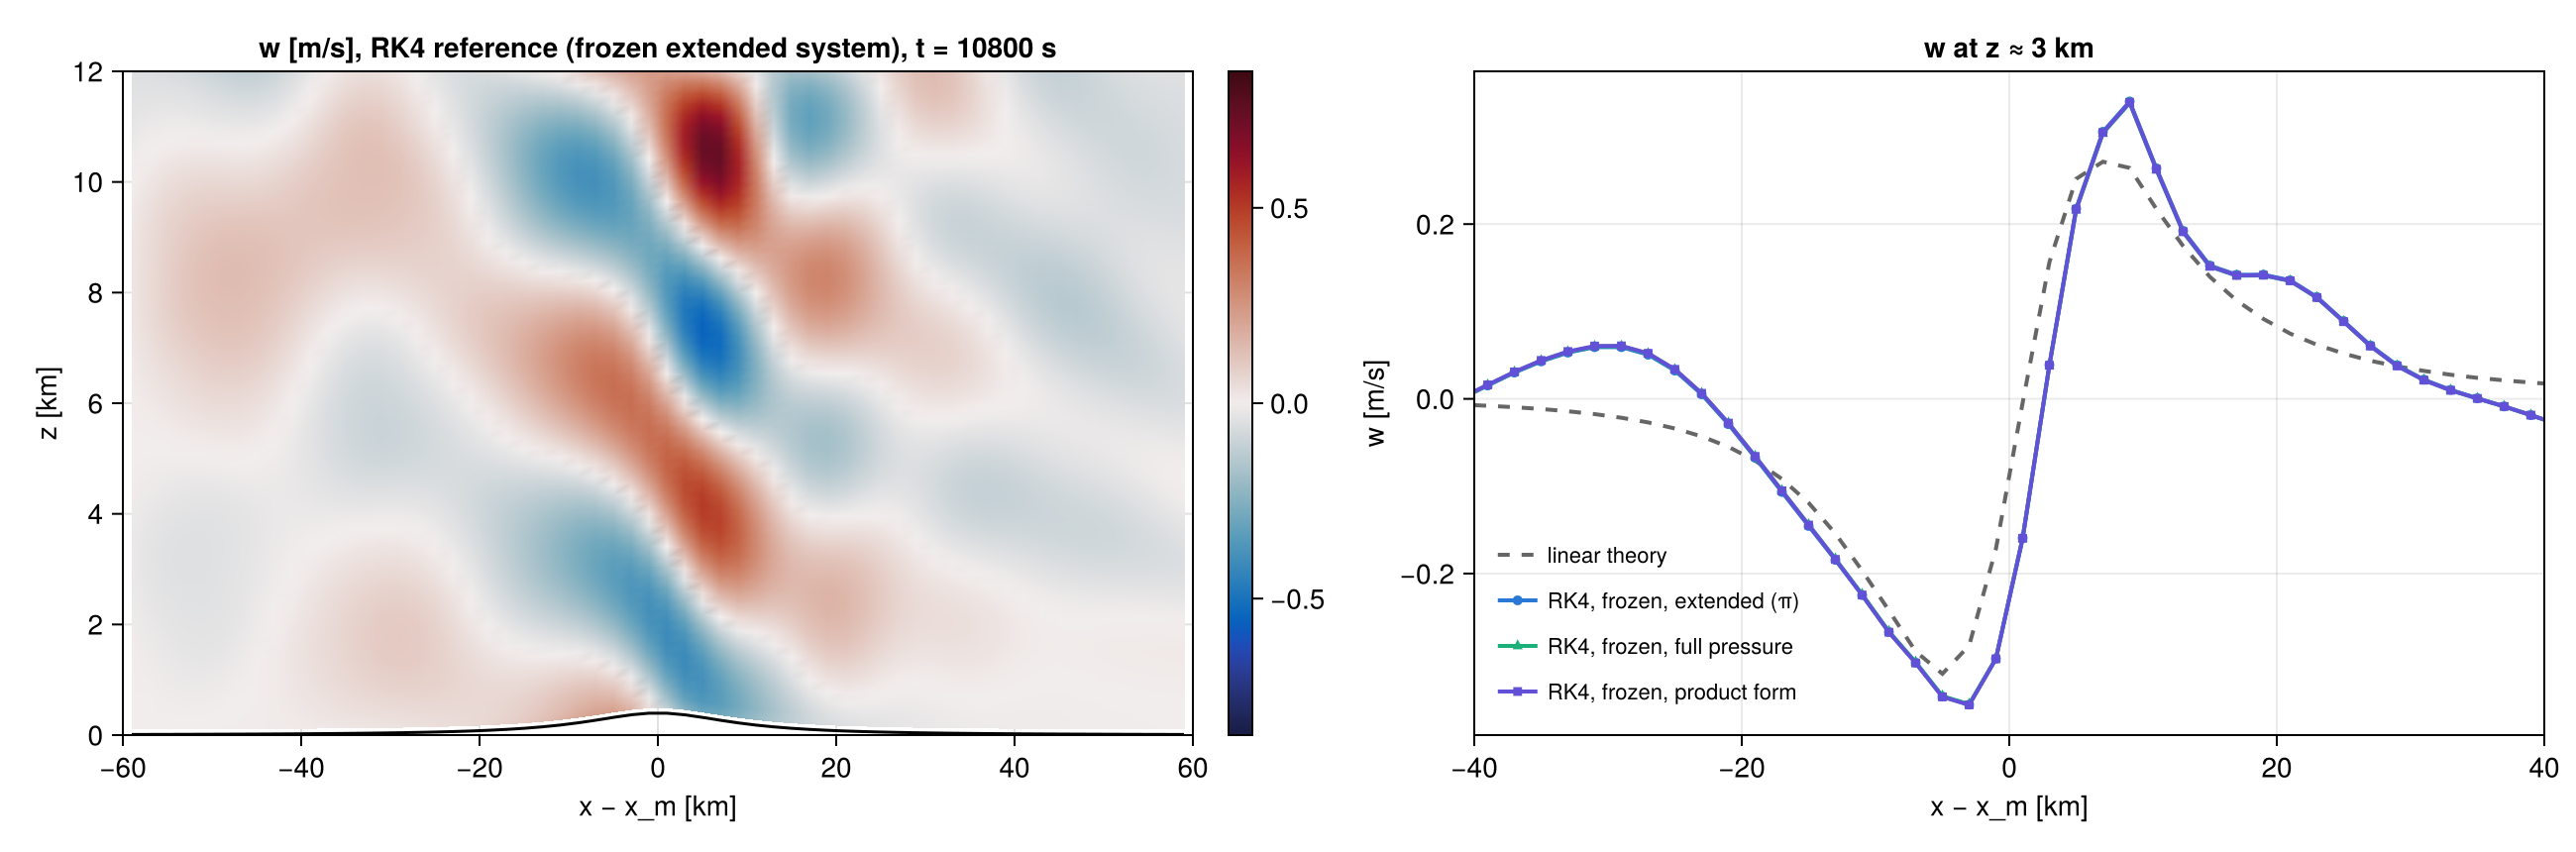
\includegraphics[width=\textwidth]{agnesi_reference.png}
\caption{Reference solution: $w$ at $t=10800$\,s (RK4, extended system), and $w$ at $z\approx3$\,km for the
three frozen operators and linear theory.}\label{fig:ref}
\end{figure}}{}

\paragraph{Reference.} The three RK4 references (one per operator; the linearized splitting has the
operator of the full-pressure form) give the same wave, $\max|w|=0.847$, 0.849, 0.849\,m/s
(Figure~\ref{fig:ref}). At $z=3$\,km the steady linear solution is reproduced in amplitude and phase
upstream and over the hill; the deviation in the lee is the not yet stationary part of the wave and
the transients of the impulsive start. The three operators agree to plotting accuracy, so the
differences in this study are caused by the time integration only.

\IfFileExists{agnesi_acoustic.png}{%
\begin{figure}[htbp]\centering
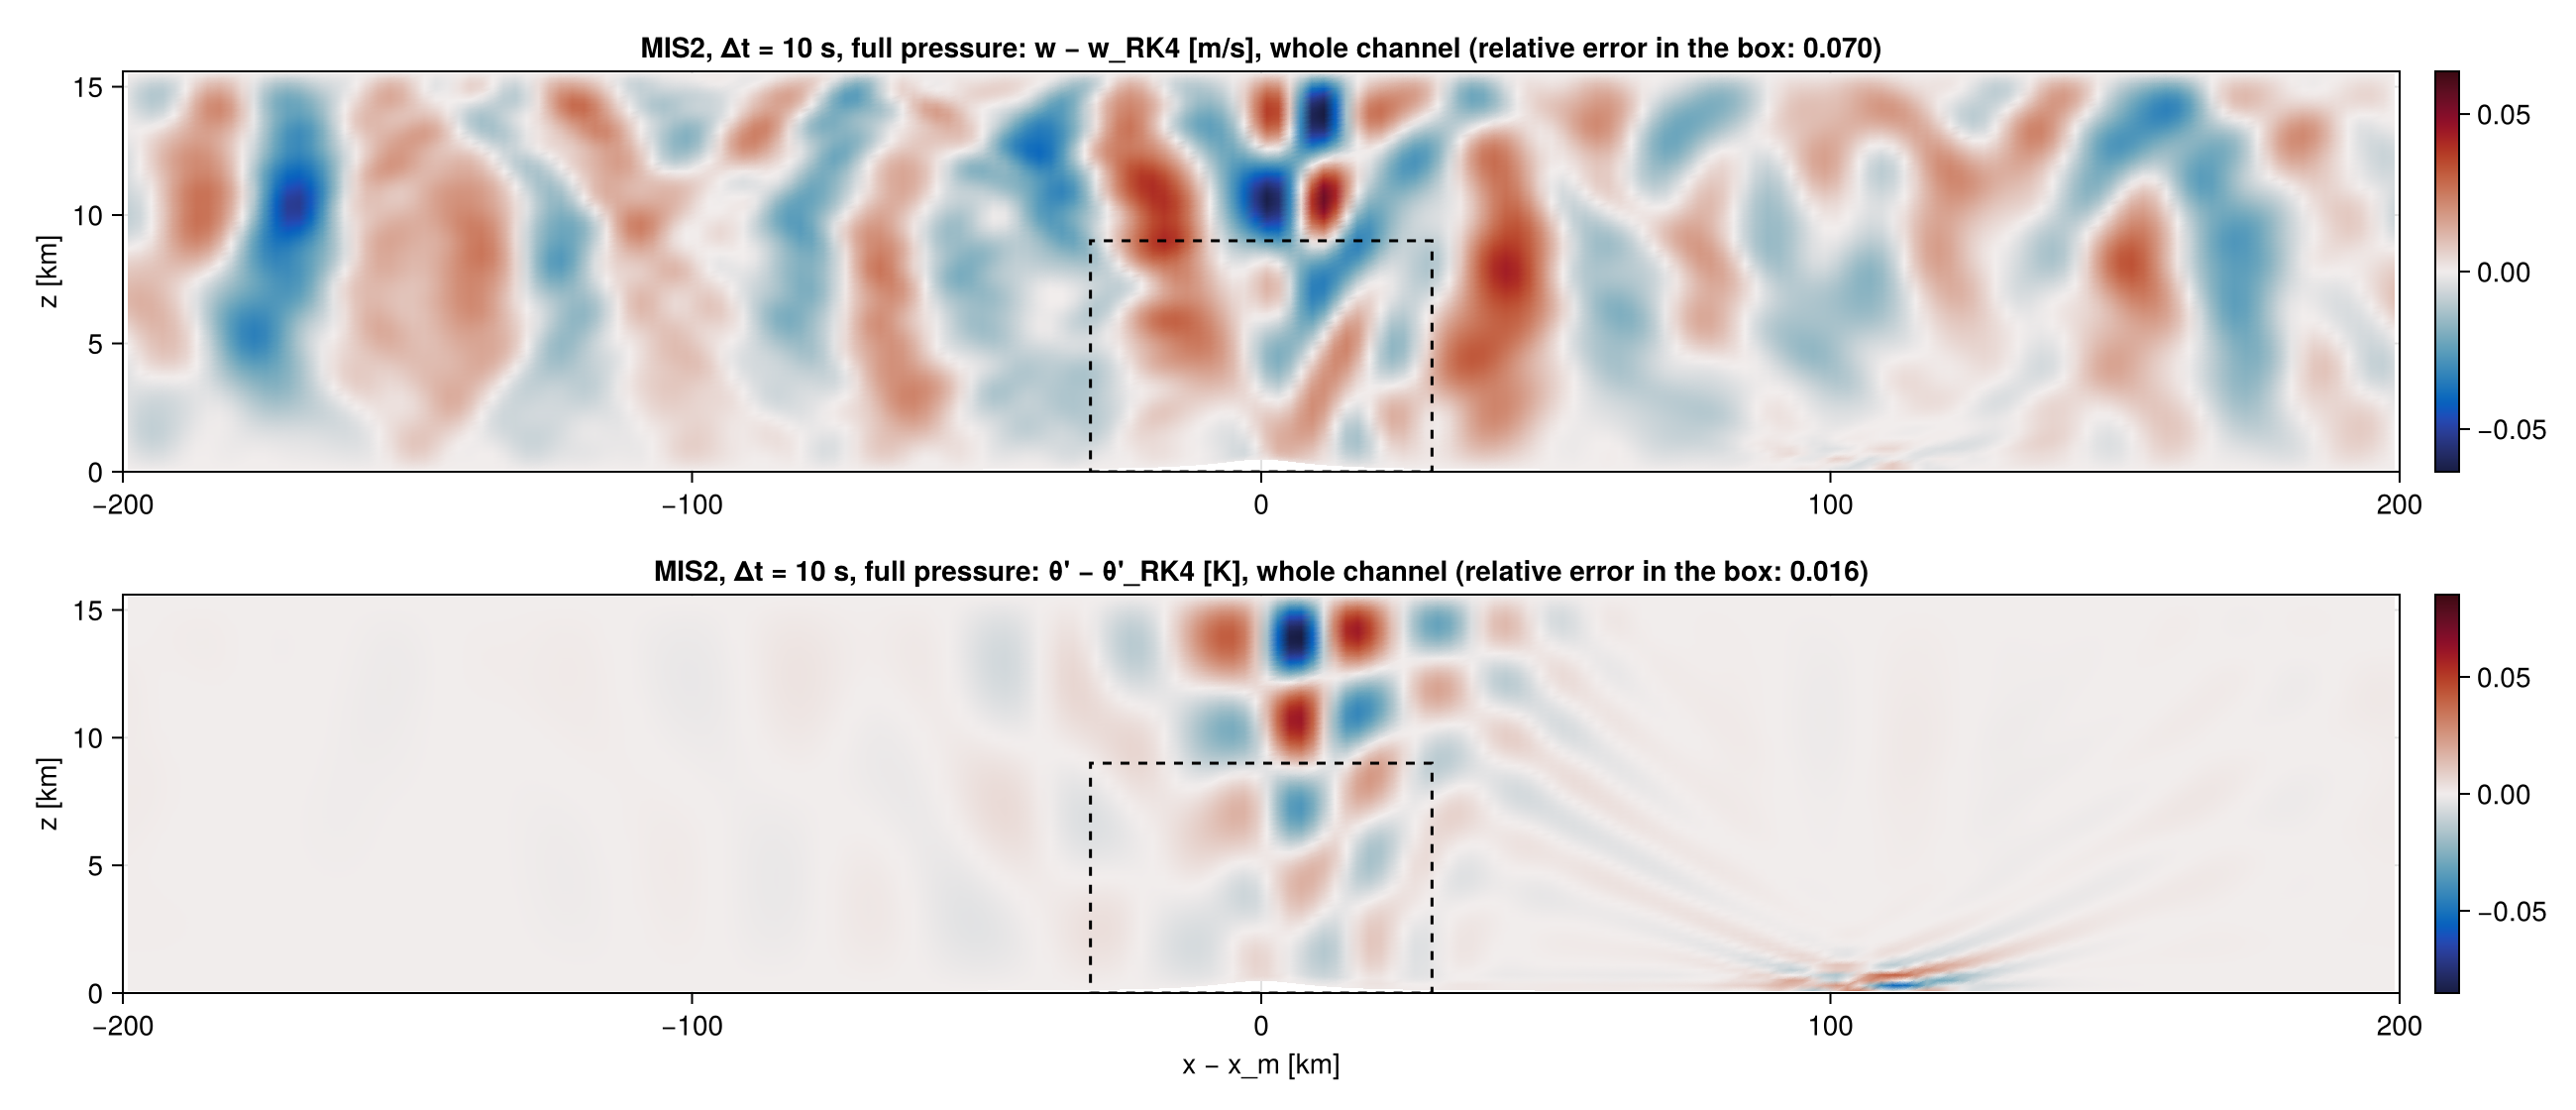
\includegraphics[width=\textwidth]{agnesi_acoustic.png}
\caption{MIS2, $\dt=10$\,s, full pressure, minus RK4 in the whole channel. Top: $w$, dominated by the
undamped vertical acoustic modes of the impulsive start; bottom: $\theta'$, the phase error of the
mountain wave above the hill. Dashed: the error box.}\label{fig:acoustic}
\end{figure}}{}

\paragraph{Small time steps.} With $n_{\rm sub}=\lceil\dt/\Delta\tau_{\rm ac}\rceil$ the small step is
3.3--4.3\,s for every $\dt$; for small $\dt$ the error is that of the fast integrator. All stable
methods give a $\theta'$ error of 1.2--1.9\,\% at $\dt=10$\,s, Lawson4 0.7\,\%. It falls with $\Delta\tau$:
MIS2 0.016 ($\dt=10$\,s, $\Delta\tau=3.3$\,s), 0.0071 ($\dt=5$\,s, $\Delta\tau=2.5$\,s), 0.0017
($\dt=\Delta\tau=2.5$\,s); MIS3C at $\dt=5$\,s 0.0045 and, with four times as many small steps, 0.0008.

\IfFileExists{agnesi_error_dt.png}{%
\begin{figure}[htbp]\centering
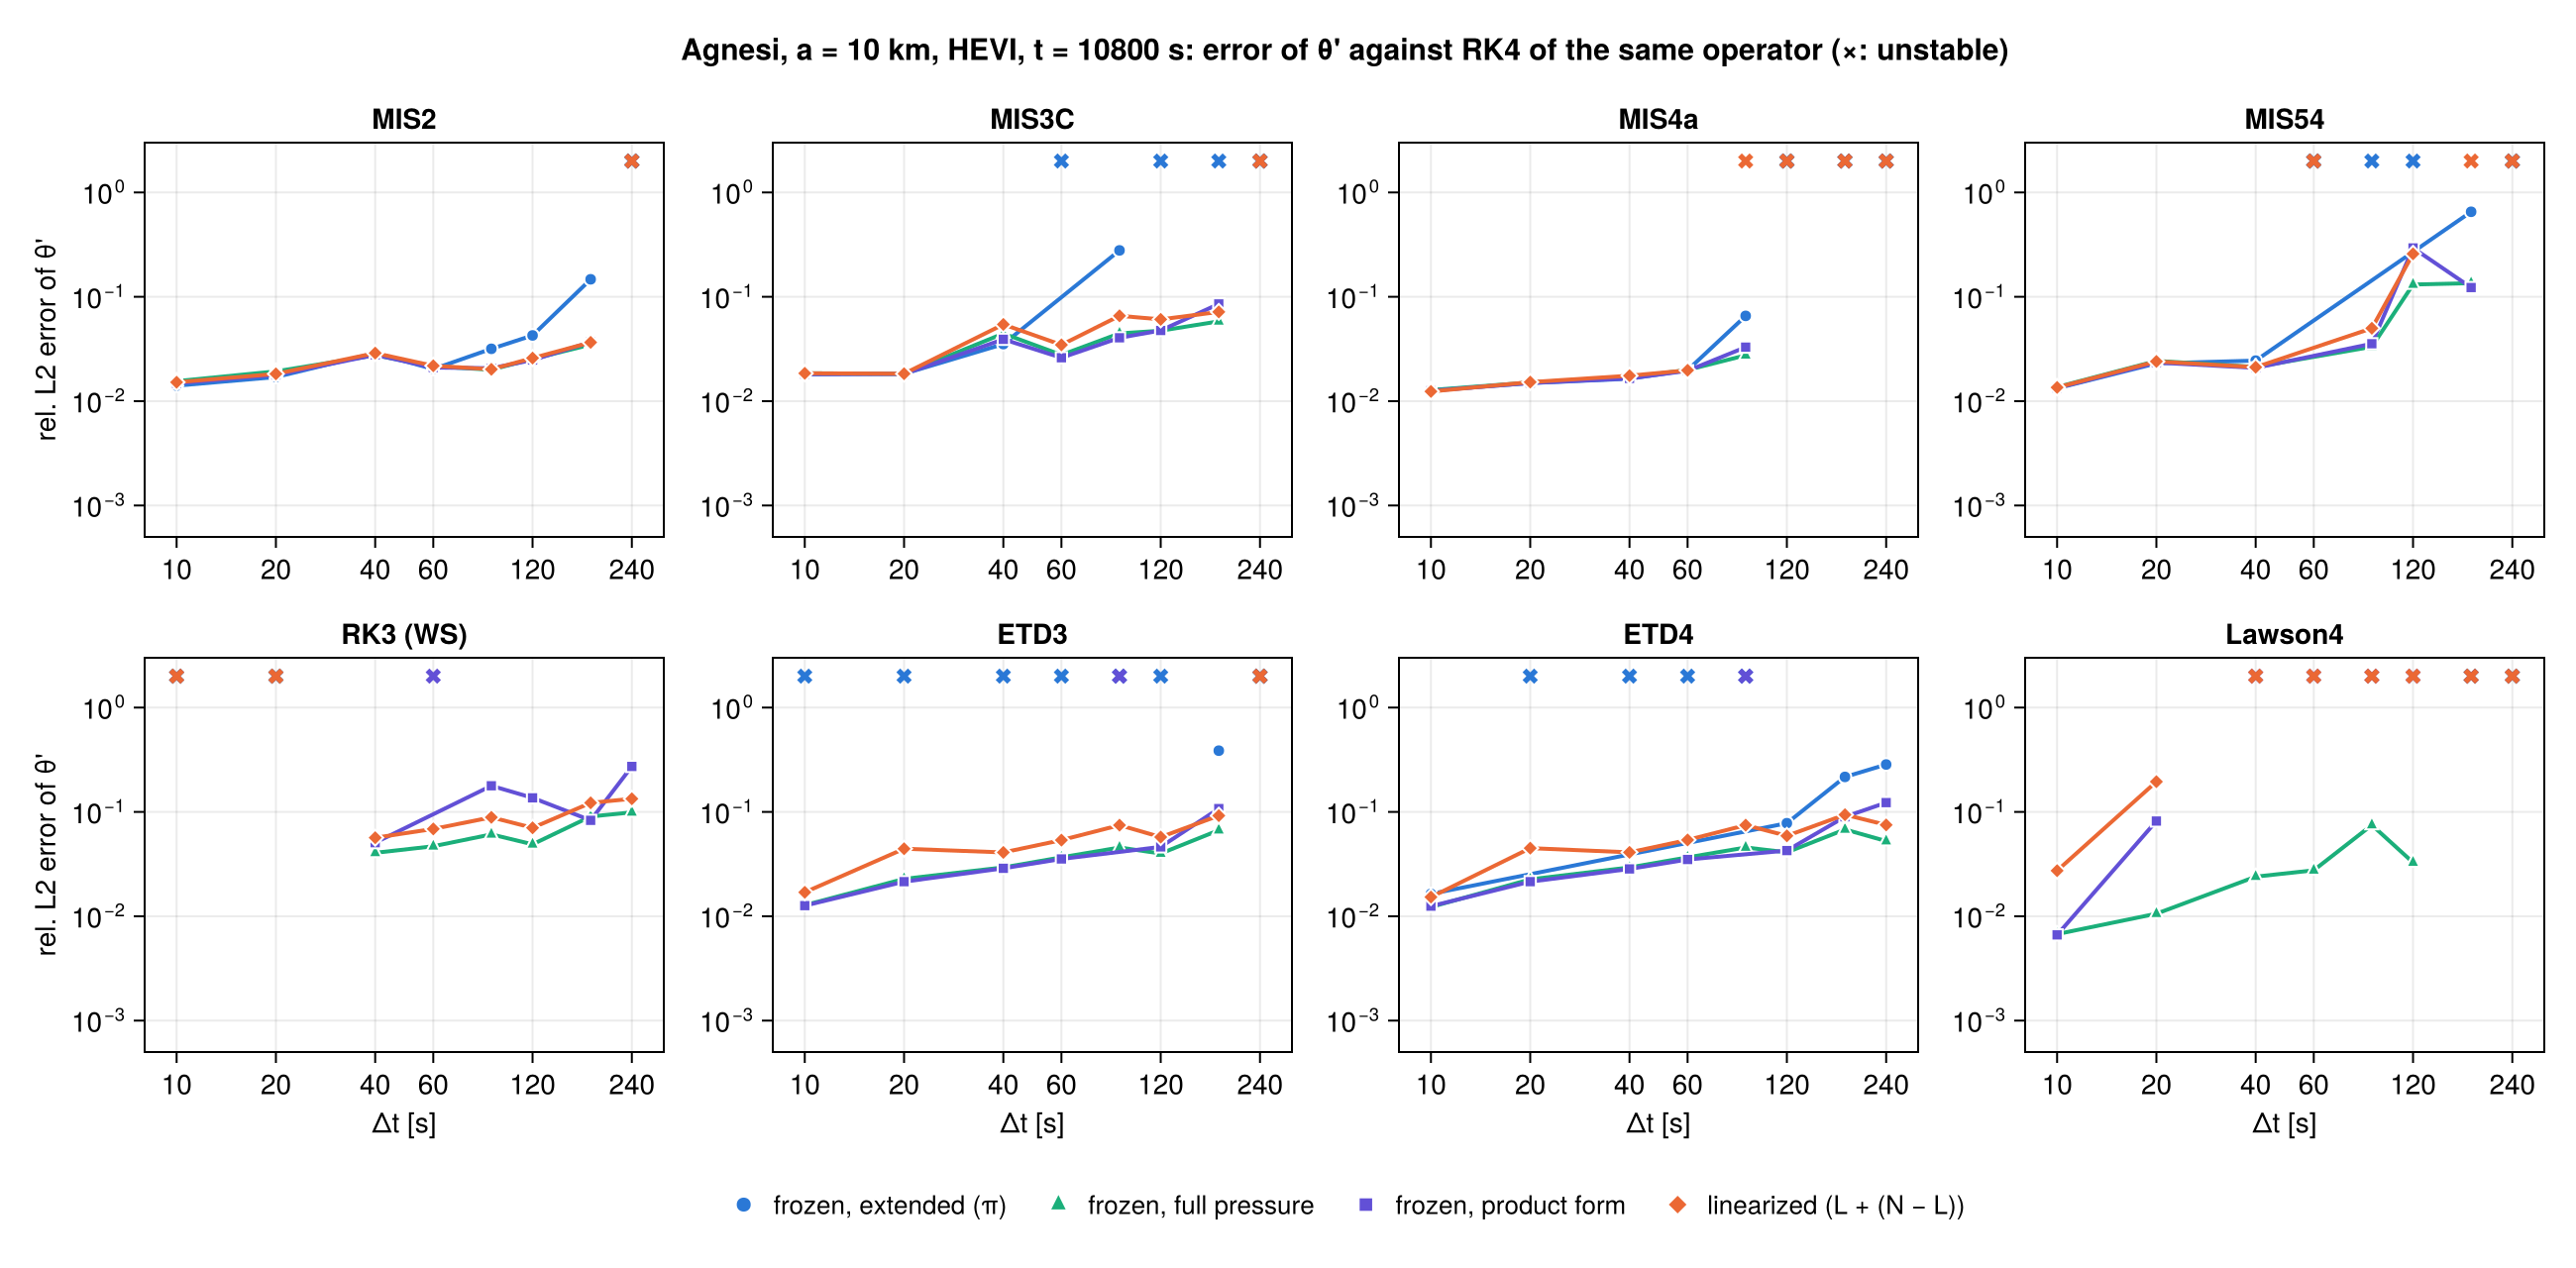
\includegraphics[width=\textwidth]{agnesi_error_dt.png}
\caption{Relative $L^2$ error of $\theta'$ against $\dt$, one panel per method, one line per
splitting: the three frozen splittings in blue, green and violet, the linearized splitting in
orange; $\times$: unstable. $n_{\rm sub}=\lceil\dt/4.3\,\mathrm s\rceil$.}\label{fig:errdt}
\end{figure}}{}

\paragraph{Errors.} Relative $L^2$ error of $\theta'$ ($n_{\rm sub}=\lceil\dt/4.3\,\mathrm s\rceil$;
u: unstable, i.e.\ non-finite or $\max|w|>17$\,m/s within $T$):
\begin{center}\small\setlength{\tabcolsep}{4pt}
\IfFileExists{tab_error_theta.tex}{\begin{tabular}{lcccccccc}\toprule
$\dt$ [s] & 10 & 20 & 40 & 60 & 90 & 120 & 180 & 240\\
$C_{\rm sound}=c\dt/\Delta x$ & 1.8 & 3.6 & 7.3 & 10.9 & 16.4 & 21.8 & 32.7 & 43.7\\
$C_{\rm adv}=U\dt/\Delta x$ & 0.05 & 0.1 & 0.2 & 0.3 & 0.45 & 0.6 & 0.9 & 1.2\\\midrule
\tabinput{tab_error_theta.tex}
\bottomrule\end{tabular}}{}
\end{center}

The error grows only slowly with $\dt$: MIS2 goes from 1.6\,\% at $\dt=10$\,s to 3.5\,\% at 180\,s for
the full-pressure form, i.e.\ at fixed $\Delta\tau$ the large step contributes little to the error.
In the stable range the three $p$-based splittings (full pressure, product form, linearized) give
practically the same MIS errors; the differences are in the stability. The frozen and linearized
splittings differ most for the methods whose fast stages start from $q^n$ and use a fast part
frozen at $q^n$ (ETD, Lawson, RK3): the frozen full-pressure form is about 30\,\% more accurate than the
linearized one for RK3, ETD3 and ETD4 (e.g.\ ETD4, $\dt=60$\,s: 0.037 against 0.054). The reason is that
the frozen full-pressure fast part evaluates $p(\Theta)$ along the fast trajectory, while $L_n$
linearizes it at $q^n$.

\paragraph{Large time step.} Largest $\dt$ [s] with a $\theta'$ error below 10\,\% (``--'': none):
\begin{center}\small
\IfFileExists{tab_dtmax.tex}{\begin{tabular}{lcccc}\toprule
& frozen, $\pi$ & frozen, $p$ & frozen, product & linearized\\\midrule
\tabinput{tab_dtmax.tex}
\bottomrule\end{tabular}}{}
\end{center}
Observations:
\begin{itemize}
\item \textbf{MIS2 and MIS3C} are stable and accurate up to $\dt=180$\,s ($C_{\rm sound}=33$,
$C_{\rm adv}=0.9$) in all three $p$-based splittings, and fail at 240\,s ($C_{\rm adv}=1.2$), presumably
the advective limit of the slow part with third-order upwind fluxes.
\item \textbf{MIS4a} is the most accurate MIS method below its limit but fails from $\dt=120$\,s on
($C_{\rm sound}\ge22$) in every splitting, in the linearized one already at 90\,s. This matches the Knoth--Wensch stability chart of MIS4a,
whose stable advective range collapses for large sound Courant numbers.
\item \textbf{MIS54} has gaps: unstable at $\dt=60$\,s in every splitting, stable at 90\,s, inaccurate
(13--29\,\%) from 120\,s on. The instability at 60\,s persists with 2, 4 and 8 times as many small steps
(full pressure and extended system), so it belongs to the method with (nearly) exact fast stages,
not to the fast integrator: a
resonance of the stage lengths $d_i\dt$ with the gravity-wave and acoustic frequencies of the
discrete system. The error field at 120\,s (Figure~\ref{fig:diff}) is a regular, nearly
monochromatic pattern, a weakly growing mode.
\item \textbf{RK3 (WS)} is unstable at $\dt=10$ and 20\,s ($C_{\rm adv}\le0.1$) and stable from 40\,s
on, up to 240\,s. This is the behaviour predicted by the stability theory: with $\alpha=\gamma=0$ the
acoustic amplification factor has $|g_0|=1$, and the second-order term grows for small $C_{\rm adv}$
(without divergence damping, which is not used here). At large $\dt$ the advective damping of
the third-order upwind slow part suffices. Its error is 1.5--3 times the MIS2 error at the same
$\dt$.
\item \textbf{ETD3, ETD4} are stable in the $p$-based splittings up to 180--240\,s with errors between
MIS2 and RK3, at 2.1--2.5 times the fast work of MIS2. In the product form they fail at
$\dt=90$\,s (a gap similar to MIS54).
\item \textbf{Lawson4} works only with the full nonlinear fast part (full pressure) up to 120\,s; with
the product form or the linearized fast part it fails from $\dt=40$\,s on. In the Lawson
method the increments $\dt\,a_{ij}\tilde S(Y_j)$ are propagated by the fast flow between the nodes;
with a fast part linear in $z$ that is not the linearization of $N$ along the solution, the
propagated increments do not cancel, and the defect is amplified by the fast flow.
\item \textbf{The extended system} (frozen, $\pi$) is the least robust: RK3, ETD3 and Lawson4 are unstable
at almost every $\dt$, ETD4 at 20--90\,s, MIS3C and MIS54 from 60\,s on; only MIS2 (and MIS4a up to its
own limit) are as robust as for the $p$-based forms. See the discussion.
\end{itemize}

\IfFileExists{agnesi_diff_large_dt.png}{%
\begin{figure}[htbp]\centering
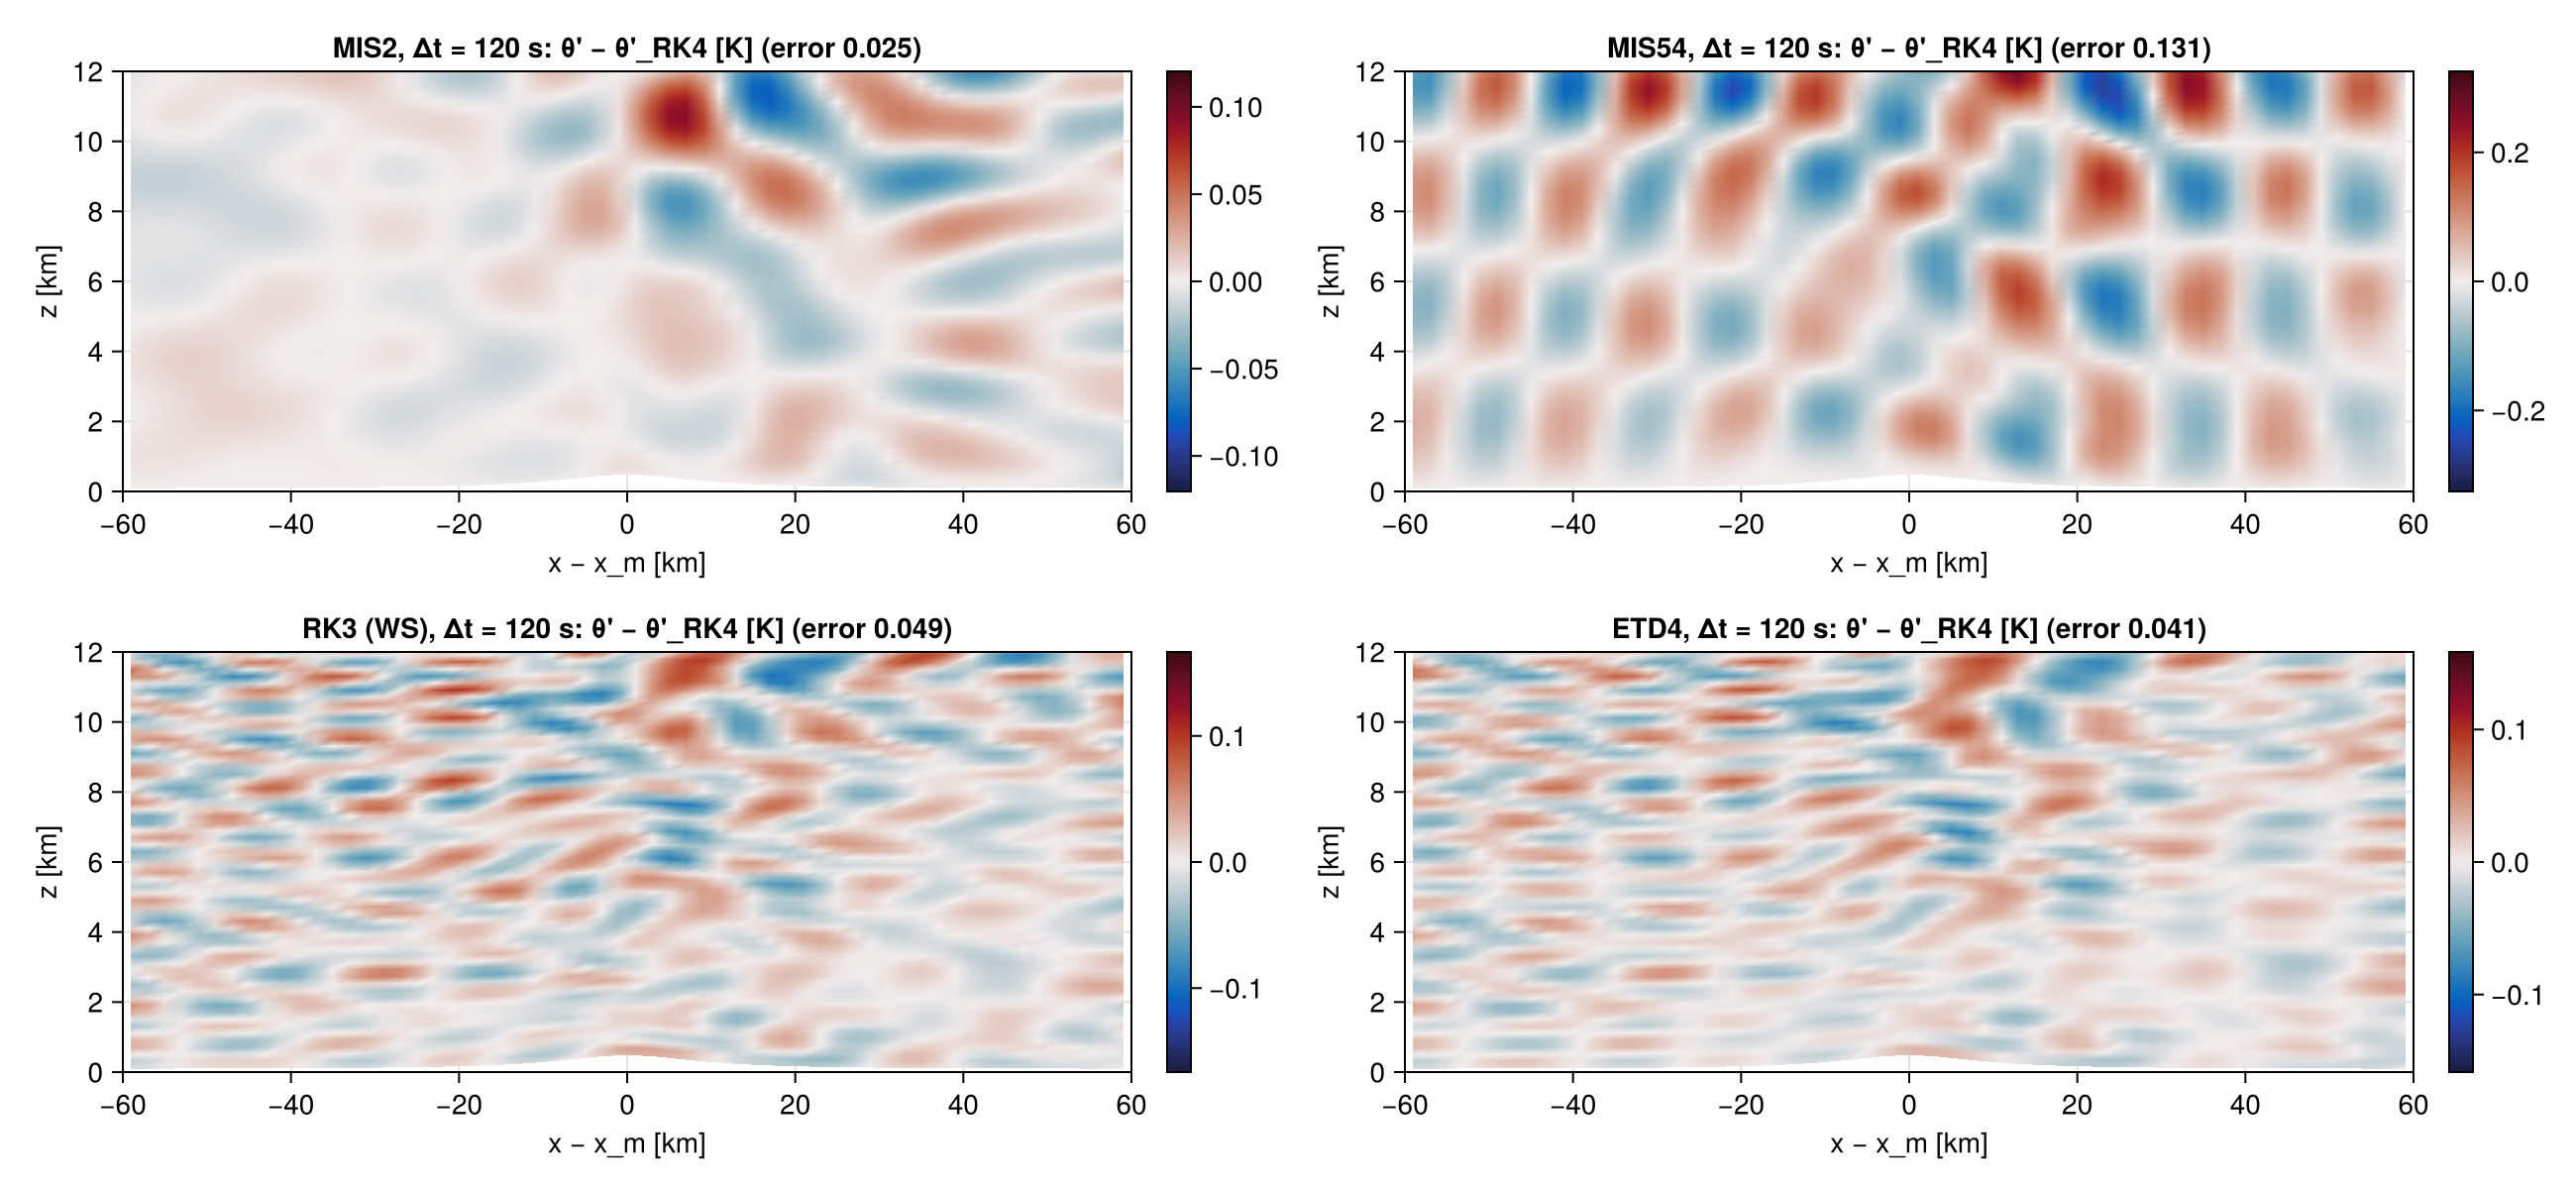
\includegraphics[width=\textwidth]{agnesi_diff_large_dt.png}
\caption{$\theta'-\theta'_{\rm RK4}$ at $\dt=120$\,s (frozen, full pressure). MIS2: smooth phase error of
the wave; MIS54: a growing regular mode near the stability limit; RK3 and ETD4: undamped small-scale
noise layered in the vertical.}\label{fig:diff}
\end{figure}}{}

The error fields at $\dt=120$\,s (Figure~\ref{fig:diff}) show the three kinds of error. MIS2 has a
smooth phase error of the wave above the hill. RK3 and ETD4 have errors of similar size, but
small-scale and layered in the vertical, everywhere in the domain: modes that are poorly resolved by
the fast integrator and are not damped, because these methods have $|g_0|=1$. MIS54 shows a regular
growing mode.

\paragraph{Number of small steps.}\label{sec:nsub} $\dt=60$\,s, $n_{\rm sub}=14\,f$ ($\Delta\tau=4.3$\,s$/f$),
$\theta'$ error:
\begin{center}\small
\IfFileExists{tab_nsub.tex}{\begin{tabular}{lcccc}\toprule
$f$ & 1 & 2 & 4 & 8\\\midrule
\tabinput{tab_nsub.tex}
\bottomrule\end{tabular}}{}
\end{center}
\IfFileExists{agnesi_error_nsub.png}{%
\begin{figure}[htbp]\centering
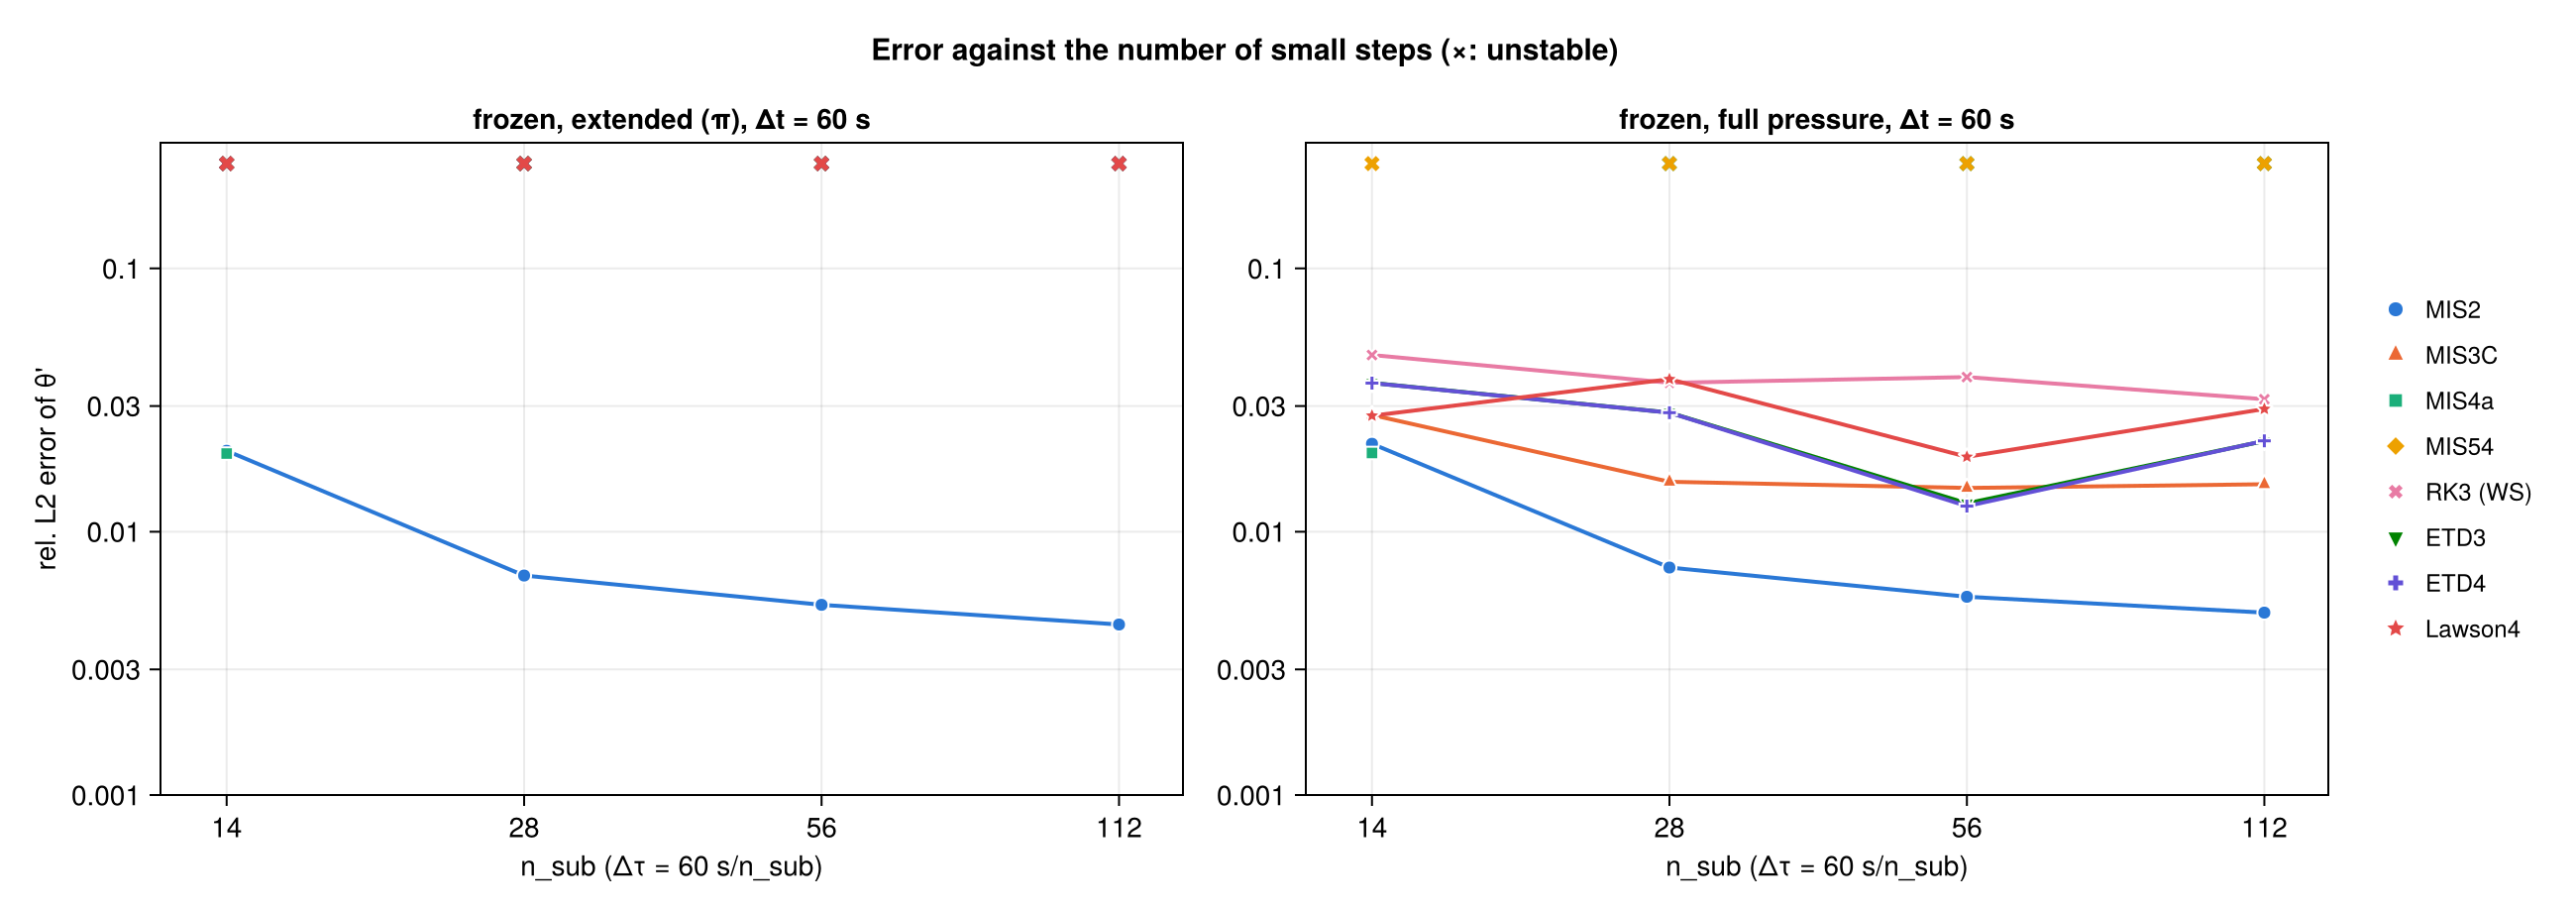
\includegraphics[width=\textwidth]{agnesi_error_nsub.png}
\caption{$\theta'$ error against the number of small steps, $\dt=60$\,s; left: extended system,
right: full pressure; $\times$: unstable.}\label{fig:nsub}
\end{figure}}{}
With the standard number of small steps ($f=1$, $\Delta\tau=4.3$\,s) the error is dominated by
the fast integrator. MIS2 drops from 0.022 to 0.0073 when the small step is halved and then saturates
at 0.005 (extended system 0.0044). That is the error of the large step $\dt=60$\,s itself, about a
quarter of the total error at $f=1$. MIS3C saturates at 0.015, a larger large-step error than MIS2.
For RK3, ETD3, ETD4 and Lawson4 the error does not decrease monotonically
(e.g.\ ETD4: 0.037, 0.028, 0.013, 0.022). These methods do not damp the poorly resolved fast modes
($|g_0|=1$), and the phase of these modes, and with it the error, depends on $n_{\rm sub}$.

MIS4a and MIS54 behave in the opposite way to the intuition ``more small steps, more accuracy'':
MIS4a is stable with $f=1$ and unstable with $f=2,4,8$, and MIS54 is unstable for every $f$. With
few small steps the fast integrator (horizontal Störmer--Verlet at acoustic Courant number 0.78,
Crank--Nicolson in the vertical) adds damping and dispersion to the high fast frequencies. With
more small steps the fast stages approach the exact flow, and $\dt=60$\,s ($C_{\rm sound}=11$) lies
outside the stability region of MIS4a and MIS54 with exact fast stages. This agrees with the
observation in the stability study that, at fixed divergence damping, more small steps weaken the
damping of the method. The stability of a split-explicit method is therefore a property of the pair
(MIS method, fast integrator with its $\Delta\tau$), and a method should be qualified with the
$n_{\rm sub}$ it is used with. The extended system with $f\ge2$ is stable only with MIS2.

%======================================================================
\section{Discussion}
\paragraph{Why MIS is robust.} The stability theory of the companion report gives the amplification
factor of a pure acoustic mode as $R(i\omega,\mu)=e^{i\omega}\sum_kg_k\mu^k$, $\mu$ the slow eigenvalue.
For RK3, ETD and Lawson $|g_0|=1$: an acoustic or poorly resolved fast mode is neither damped nor
amplified to leading order, and the next term decides. For RK3 this term amplifies for small advective
Courant numbers, which is why RK3 is unstable at $\dt\le20$\,s here and why WRF needs divergence
damping. MIS methods with $\alpha,\gamma\ne0$ have $|g_0|<1$ (MIS2, MIS3C, MIS4a: $1-|g_0|\sim\omega^4$,
MIS54: $\omega^6$), a built-in damping of the fast modes that is independent of the fast integrator.
The test confirms both sides: without any divergence damping MIS2 and MIS3C are stable from
$\dt=10$ to 180\,s in all $p$-based splittings, and the error fields at large $\dt$ are smooth for
MIS2, but contain undamped small-scale noise for RK3 and ETD4 (Figure~\ref{fig:diff}).

\paragraph{Accuracy and cost.} With $n_{\rm sub}\propto\dt$ the small step is fixed, and the error is
dominated by the fast integrator. The large step adds little: the $\theta'$ error of MIS2 doubles from
$\dt=10$ to 180\,s. The cost is the fast work, $\sum_id_i\,n_{\rm sub}$ small steps per large step:
over the run 2991 small steps for MIS2 and MIS3C, 3709 for MIS4a, 4620 for RK3, 4732 for MIS54, 6300 for
ETD3 and Lawson4, 7560 for ETD4 (each with three HEVI column solves). MIS2 has the lowest fast work, its error is within 10\,\% of
the best MIS method (MIS4a) where both are stable, and only RK3 and ETD4 reach a larger step. At
$\dt=60$\,s, ETD4 needs 2.5 times the fast work of MIS2 for 1.7 times its error, and RK3 needs 1.5
times the work for 2.1 times the error.

\paragraph{The higher-order MIS methods.} MIS4a and MIS54 are not better than MIS2 here. Their higher
order (reduced to 2 by the frozen coefficients anyway) is invisible behind the fast-integrator error.
Their stability regions have gaps at large sound Courant numbers (MIS4a from $C_{\rm sound}\approx20$,
MIS54 at $C_{\rm sound}\approx11$), which are properties of the methods with exact fast stages: more
small steps make them worse (Section~\ref{sec:nsub}). The idealized Knoth--Wensch test predicts
such limits, but not their exact positions, which depend on the frequency content of the discrete
operator (gravity waves, terrain metric).

\paragraph{The splitting.} For MIS methods the splitting hardly matters, as long as $p$ is the prognostic
pressure: full pressure, product form and linearized splitting give the same errors and the same
stability limits within one $\dt$ step of the scan. For the methods that start every stage from
$q^n$ with a fast part frozen at $q^n$ (RK3, ETD, Lawson) the frozen full-pressure form is clearly
best. It is about 30\,\% more accurate than the linearized one and is the only form in which Lawson4
works beyond $\dt=20$\,s. The product form is a poor compromise for these methods (RK3 unstable at
60\,s, ETD at 90\,s, Lawson4 from 40\,s).

\paragraph{The extended system.} The extended system with the Exner pressure is less robust than the
$p$-based forms for every method except MIS2. The cause is not the fast part: the spectra of the frozen
fast operators of the three frozen forms coincide on a reduced grid ($40\times26$ cells, same hill and
$\Delta x$, $\Delta\eta$): $\max\Re\lambda=5.3\cdot10^{-5}$\,s$^{-1}$ on the terrain grid
(machine zero on flat ground), and the same imaginary parts. The difference is in the full operator $N$:
linearized about the initial flow over the hill, the extended system has real eigenvalues up to
$1.4\cdot10^{-3}$\,s$^{-1}$, against $4.8\cdot10^{-7}$\,s$^{-1}$ for the $p$-based operators. The
eigenvectors are pure constraint defects: a perturbation $\delta\Theta$ without the consistent
$\delta\pi=\pi_\Theta\delta\Theta$ ($|\delta\pi-\pi_\Theta\delta\Theta|=31\,|\delta\pi|$), with negligible momentum, located in the lowest layer on the upslope
side. They are absent on flat ground and at $U=0$. The extended system carries an additional degree of
freedom, the defect $\pi-\pi(\Theta)$, which is neutral in the continuous equations but is not
preserved by the discrete $\pi$ equation in the sloping lowest layer, where the contravariant flux
converges. The reset $\pi\leftarrow\pi(\Theta)$ after each large step does not cure the instability
(the same runs are unstable without it), so the defect is created and amplified within the step,
by the stage combinations of the frozen coefficients. The growth rate alone ($\lambda\dt\approx0.08$ at
$\dt=60$\,s) does not explain the blow-up; we therefore regard the defect mode as the mechanism to be
removed, not as a complete explanation. Possible remedies are a $\pi$ equation that uses exactly the
discrete divergence of the $\Theta$ equation multiplied by $\pi_\Theta$ of the same cell, a
relaxation of $\pi$ towards $\pi(\Theta)$ inside the fast loop, or the full-pressure frozen form,
which has no additional variable.

\paragraph{Recommendation for this configuration.} MIS2 (or MIS3C) with the frozen full-pressure
splitting and HEVI Störmer--Verlet/Crank--Nicolson small steps at $\Delta\tau\approx0.8\,\Delta x/c$:
stable without divergence damping from $\dt=10$ to 180\,s ($C_{\rm sound}$ up to 33) with a $\theta'$
error of 2--4\,\% against RK4, at the lowest fast work of all methods tested. The accuracy is
limited by the small step, not by $\dt$. The vertical acoustic modes of the impulsive start remain
unresolved in phase by every split method; this concerns $w$, not the mountain wave.

%======================================================================
\appendix
\section{Error of $w$}
Relative $L^2$ error of $w$ in the same box. It is dominated by the vertical acoustic modes of
the impulsive start (Figure~\ref{fig:acoustic}) and therefore does not decrease with $\dt$:
\begin{center}\small\setlength{\tabcolsep}{4pt}
\IfFileExists{tab_error_w.tex}{\begin{tabular}{lcccccccc}\toprule
$\dt$ [s] & 10 & 20 & 40 & 60 & 90 & 120 & 180 & 240\\\midrule
\tabinput{tab_error_w.tex}
\bottomrule\end{tabular}}{}
\end{center}

%======================================================================
\begin{thebibliography}{99}
\bibitem{bauer} S.~Bauer, O.~Knoth: Extended multirate infinitesimal step methods: derivation of order
conditions. J.\ Comput.\ Appl.\ Math.\ 387 (2021), 112541.
\bibitem{coxmatthews} S.M.~Cox, P.C.~Matthews: Exponential time differencing for stiff systems.
J.\ Comput.\ Phys.\ 176 (2002), 430--455.
\bibitem{galchen} T.~Gal-Chen, R.C.J.~Somerville: On the use of a coordinate transformation for the
solution of the Navier--Stokes equations. J.\ Comput.\ Phys.\ 17 (1975), 209--228.
\bibitem{gallus} W.A.~Gallus, J.B.~Klemp: Behavior of flow over step orography. Mon.\ Wea.\ Rev.\ 128
(2000), 1153--1164.
\bibitem{hlw} E.~Hairer, C.~Lubich, G.~Wanner: Geometric Numerical Integration, 2nd ed. Springer 2006.
\bibitem{hicken} J.E.~Hicken, F.E.~Ham, J.~Militzer, M.~Koksal: A shift transformation for fully conservative
methods: turbulence simulation on complex, unstructured grids. J.\ Comput.\ Phys.\ 208 (2005), 704--734.
\bibitem{hochbruck} M.~Hochbruck, A.~Ostermann: Exponential integrators. Acta Numerica 19 (2010), 209--286.
\bibitem{jaehn} M.~J\"ahn, O.~Knoth, M.~K\"onig, U.~Vogelsberg: ASAM v2.7: a compressible atmospheric
model with a Cartesian cut cell approach. Geosci.\ Model Dev.\ 8 (2015), 317--340.
\bibitem{klempwil} J.B.~Klemp, R.B.~Wilhelmson: The simulation of three-dimensional convective storm
dynamics. J.\ Atmos.\ Sci.\ 35 (1978), 1070--1096.
\bibitem{ksd} J.B.~Klemp, W.C.~Skamarock, J.~Dudhia: Conservative split-explicit time integration methods
for the compressible nonhydrostatic equations. Mon.\ Wea.\ Rev.\ 135 (2007), 2897--2913.
\bibitem{ksh} J.B.~Klemp, W.C.~Skamarock, S.-H.~Ha: Damping acoustic modes in compressible horizontally
explicit vertically implicit (HEVI) and split-explicit time integration schemes. Mon.\ Wea.\ Rev.\ 146
(2018), 1911--1923.
\bibitem{knothwensch} O.~Knoth, J.~Wensch: Generalized split-explicit Runge--Kutta methods for the
compressible Euler equations. Mon.\ Wea.\ Rev.\ 142 (2014), 2067--2081.
\bibitem{bseries} O.~Knoth, J.~Wensch: B-series and split-explicit methods. Manuscript,
\url{https://github.com/OsKnoth/B-Series}.
\bibitem{krogstad} S.~Krogstad: Generalized integrating factor methods for stiff PDEs. J.\ Comput.\ Phys.\
203 (2005), 72--88.
\bibitem{lawson} J.D.~Lawson: Generalized Runge--Kutta processes for stable systems with large Lipschitz
constants. SIAM J.\ Numer.\ Anal.\ 4 (1967), 372--380.
\bibitem{sk92} W.C.~Skamarock, J.B.~Klemp: The stability of time-split numerical methods for the
hydrostatic and the nonhydrostatic elastic equations. Mon.\ Wea.\ Rev.\ 120 (1992), 2109--2127.
\bibitem{sk94} W.C.~Skamarock, J.B.~Klemp: Efficiency and accuracy of the Klemp--Wilhelmson
time-splitting technique. Mon.\ Wea.\ Rev.\ 122 (1994), 2623--2630.
\bibitem{wkg} J.~Wensch, O.~Knoth, A.~Galant: Multirate infinitesimal step methods for atmospheric flow
simulation. BIT Numer.\ Math.\ 49 (2009), 449--473.
\bibitem{ws} L.J.~Wicker, W.C.~Skamarock: Time-splitting methods for elastic models using forward time
schemes. Mon.\ Wea.\ Rev.\ 130 (2002), 2088--2097.
\end{thebibliography}
\end{document}
